\section{Implementation Details}
\label{sec:implement}

\begin{figure}[htbp]
\centering
\label{fig:fsinfs}
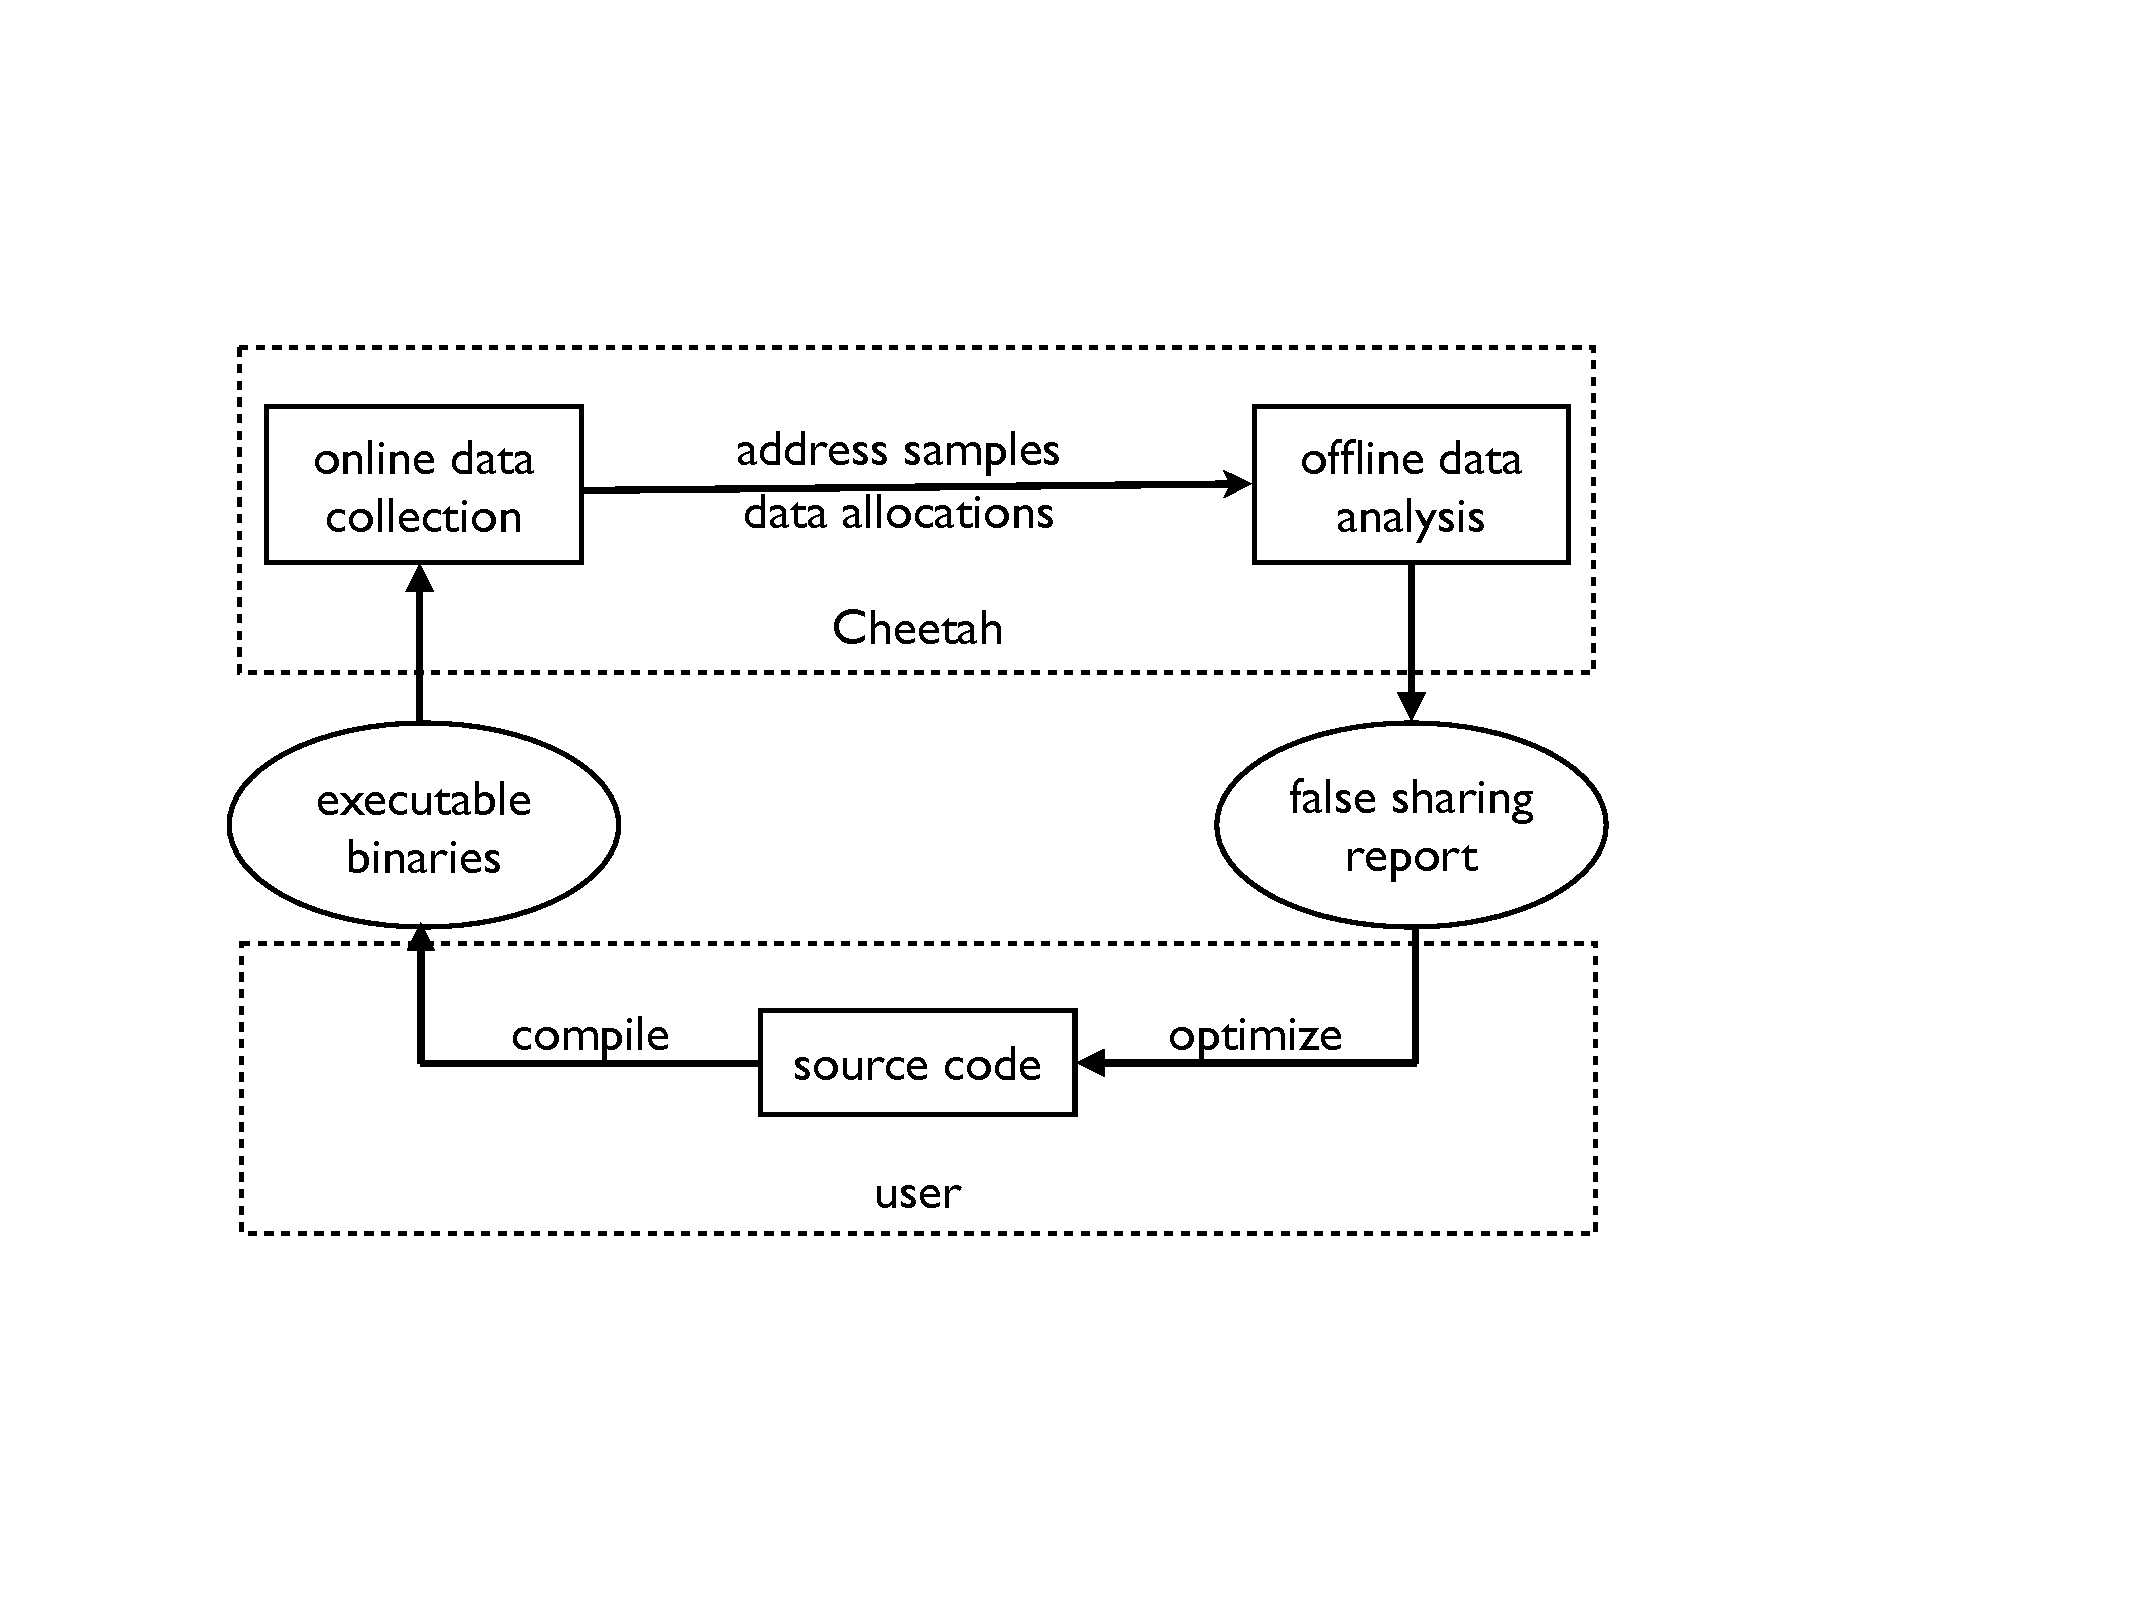
\includegraphics[width=\columnwidth]{figure/workflow}
\caption{The workflow of \cheetah{}}
\end{figure}

In this section, we describe the implementation of \cheetah{} and highlight our solutions in addressing technical challenges. Figure~\ref{} shows the workflow of \cheetah{}, 
which consists of an online and offline components. We elaborate these components in the rest of this section.

\subsection{Online Component}
The online component of \cheetah{} intercepts each thread by overloading the thread creation function, i.e., {\tt pthread\_create}. At meanwhile, \cheetah{} sets up the PMU for address sampling to let each thread accept samples individually. {\color{red} did you associate samples with data objects online? Is there any challenge in efficiently handling parallelism?}



\subsection{Offline Component}
{\color{red} How to merge all of the analysis results from different threads? What if there are many threads? How is the scalability of the analysis? What's the output? You can have a forward pointer to Section 6.}


\begin{comment}


This section presents the detailed implementation of \Cheetah{}'s detection: it first describes how to sample memory accesses (in Section~\ref{sec:detect-trace}) and how to compute the number of cache invalidations based on the pattern of memory accesses (see Section~\ref{sec:compute}); then we describes how to report false sharing precisely and correctly (see Section~\ref{sec:report});

%\redmark{Should we add a figure about different components??}

\subsection{Sampling Memory Accesses}
\label{sec:detect-trace}
% How to trace the memory accesses?
% What is the benefit of using performance counter, non-instrusive
% What information that we can get about an memory access
% How we will handle this information? We will pass it to cache invalidations module

As described in Section~\ref{sec:perfcounter}, \Cheetah{} relies on hardware performance counters, such as AMD's IBS registers, to sample memory accesses. Hardware performance counters provide a non-intrusive and efficient approach to track memory accesses. \Cheetah{} is a library that can be preloaded before the execution of an application: there is no need to change or recompile the programs, or to modify the underlying operating system. 

\cheetah{} performs its initialization before running an application, by putting it into the constructor attribute. During the initialization, \Cheetah{} installs a signal handler so that it can collect detailed information of memory accesses after a specified sample period. In order to simplify the signal handling, \Cheetah{} also configures the signal handler to be responded by the current thread, by calling \texttt{fcntl} function with \texttt{F\_SETOWN\_EX} flag. \cheetah{} also sets up the custom allocator and its internal heap in the initialization.  

Inside the signal handler, \Cheetah{} collects detailed information of every sampled memory access, including memory address, thread id, read or write operation, and access latency, which can be fed into the computing module to compute the number of cache invalidations and the prediction module to predict performance impact. 

\subsection{Computing Cache Invalidations}
\label{sec:compute}

\Cheetah{} computes possible cache invalidations on each cache line based on the rule that is described in Section~\ref{sec:computeinvalidations}. \Cheetah{} maintains a two-entries-cache-history table for each cache line and checks against the history table to decide whether an access leads to a cache invalidation. In order to locate the cache history of each cache line, \Cheetah{} implements the shadow memory for all virtual addresses, which has been introduced before~\cite{qinzhao}. 

Since \cheetah{} only cares about those cache lines that can potentially involve in false sharing. We observe that only those cache lines with a big number of writes can possibly cause a lot of cache invalidations. Based on this observation, cache lines with a small number of writes are never be a target that can cause serious performance problem. For this reason, \Cheetah{} only tracks those cache lines when the number of writes on a cache line is larger than a pre-defined threshold, which we refer to as the {\it Tracking-Threshold}. Before this threshold is reached, \Cheetah{} only tracks the number of writes on a cache line while skipping tracking reads. This mechanism reduces performance and memory overhead at the same time.

In the implementation, \Cheetah{} maintains two arrays in the shadow memory: {\it CacheWrites} tracks the number of memory writes on every cache line, and {\it CacheTracking} tracks detailed information for each cache line. To save memory, {\it CacheTracking} for a particular cache line is allocated dynamically once the number of writes on this cache line exceeds the {\it Tracking-Threshold}. The history table, number of cache invalidations on a cache line, and detailed memory accesses are actually included in {\it CacheTracking}. These information are going to be checked in the reporting phase that is described in Section~\ref{sec:report}.
 
 \subsection{Reporting False Sharing}
% How we will report false sharing precisely and correctly?
% How we 
\label{sec:report}

\Cheetah{} aims to report false sharing correctly and precisely, same as existing work~\cite{sheriff, Predator}. \Cheetah{} will invoke the process of checking and reporting false sharing problems, either at the end of programs or receiving the instructions from users through the \texttt{SIGUSR2} signal.  

\paragraph{Correct Detection:} \Cheetah{} keeps track of word-based (four bytes) memory accesses on susceptible cache lines: how many reads or writes occurs by which thread on each word. When more than one thread access a word, \Cheetah{} marks this word to be shared. By identifying accesses on each word on a susceptible cache line, we can easily differentiate false sharing from true sharing, as shown in Figure~\ref{fig:falsesharing}. Word-based information can also help diagnose false sharing problems more detailed, which helps programmers to decide how to padding an existing data structure in order to avoid false sharing.  Because it is possible for a thread, particularly the main thread, to allocate an object and do some initialization before passing to different threads,  \cheetah{} only checks memory access inside parallel phases to avoid this problem.

\paragraph{Precise Detection.} \Cheetah{} reports precise information for global variables and heap objects that are involved in false sharing. For global variables, \Cheetah{} reports names and addresses by searching through the ELF symbol table. For heap objects, \Cheetah{} reports the lines of code for allocating these objects.  
Thus, \Cheetah{} intercepts all memory allocations and de-allocations and utilizes \texttt{backtrace()} to obtain the whole callsite stack. During the real implementation, we tried to keep the overhead of getting the callsite stack as little as possible. \cheetah{} utilizes a global hash table to save those known callsite stack. The combination of ``rip'' (instruction pointer) and ``stack offset'' is considered as the key of this global hash table. If the combination of these two values (as the key) have existed in the global hash table, we simply copied the saved callsite stack to a new object. Otherwise, backtrace() is called to fetch the callstack.  

\end{comment}
%However, it is straightforward to solve such false sharing problems by using an allocator like Hoard that avoids this kind of false sharing.


%\subsection{Predicting False Sharing}
% What is the basic idea to predict false sharing problem?
% What is the difference with Predator{}?
% For those predicted false sharing, we cannot predict performance improvement?



 